\section{Presentation of Experimental or Analytical Results/Descriptions of Final Constructed Product}

In this section, we discuss the testing outcomes of our models and explore areas for further improvement.

\subsection{Validating Model Accuracy on a Test Set}

After training, the models were evaluated on a specially prepared test set to measure their accuracy. The accuracy is defined as the proportion of samples for which the model's predictions match the actual labels.

The table and figure below present the accuracy of the model across different categories:

\begin{figure}[H]
    \centering
    \begin{minipage}{0.45\textwidth}
        \centering
        \captionof{table}{Model Accuracy on Test Set}
        \begin{tabular}{cc}
            \toprule
            Category & Accuracy(\%) \\
            \midrule
            Normal & 98.4 \\
            Horizontal Line & 95.6 \\
            Vertical Line & 80.0 \\
            Slope & 96.1 \\
            Other & 95.2 \\
            \bottomrule
        \end{tabular}
        \label{tab:model_accuracy}
    \end{minipage}
    \begin{minipage}{0.45\textwidth}
        \centering
        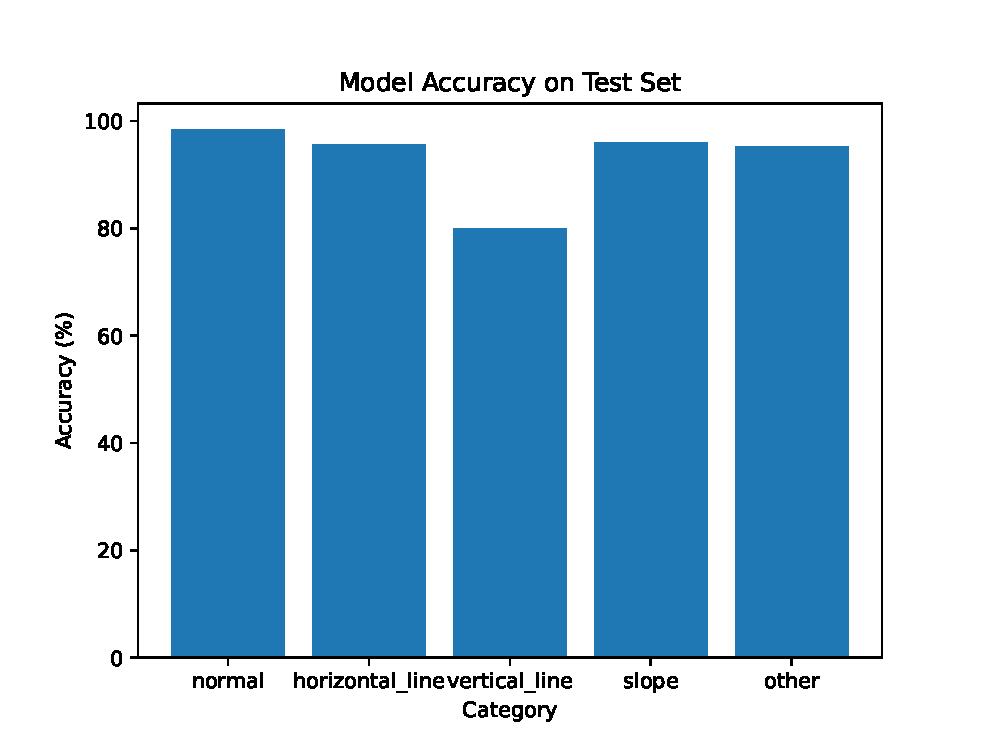
\includegraphics[width=\textwidth]{./fig/assistplot/accuracy.eps}
        \captionof{figure}{Model Accuracy on Test Set}
        \label{fig:accuracy_histogram}
    \end{minipage}
\end{figure}

\textbf{Analysis of Model Performance}
The model performs exceptionally well for the 'Normal' category with an accuracy of 98.4\%, indicating its robust capability in identifying tissue sections without significant defects. Similarly, high accuracy scores are noted for 'Horizontal Line' and 'Other' categories, reflecting the model’s effectiveness in recognizing these specific types of imperfections.

However, the accuracy for the "Vertical Line" category is significantly lower, at 80.0\%. This indicates that the model's ability to recognize this type of defect needs to be strengthened. This could be due to insufficient training data, which limits the model's learning. It could also be because the features of vertical lines are relatively less obvious, making it difficult for the model to accurately extract features.

\subsection{Improvement of the Model (Changing Input Resolution)}

Here we discuss the potential for further improvement of the model.

Rescaling high-resolution images to the default size of 299x299, as required by the InceptionV3 model, can indeed result in the loss of information and detail. This is particularly crucial for images originally at much higher resolutions, such as those captured by the VHX7000 device at 2880x2160. Directly scaling down these images may hinder the model's ability to capture all subtle differences, which is especially detrimental in fields like medical imaging where detail richness is paramount.

One potential solution is to modify the model's input layer to accept larger image sizes. This approach allows the model to process higher resolution images, thus retaining more original information and detail, which could lead to improved performance and higher accuracy. The InceptionV3 architecture, with its multiple convolutions of varying kernel sizes, is particularly well-suited to handle larger images as it can capture features at different scales effectively.

Due to the limitations imposed by the lab's hardware (16GB of VRAM), the images are rescaled to 0.4 times their original size, resulting in dimensions of 1152x864 for this experiment.

\textbf{Training the New Model (Model 4)}

Model 4 is trained with these adjusted image sizes, and its training effectiveness is as follows:

\begin{figure}[H]
    \centering
    \begin{minipage}{0.45\textwidth}
        \centering
        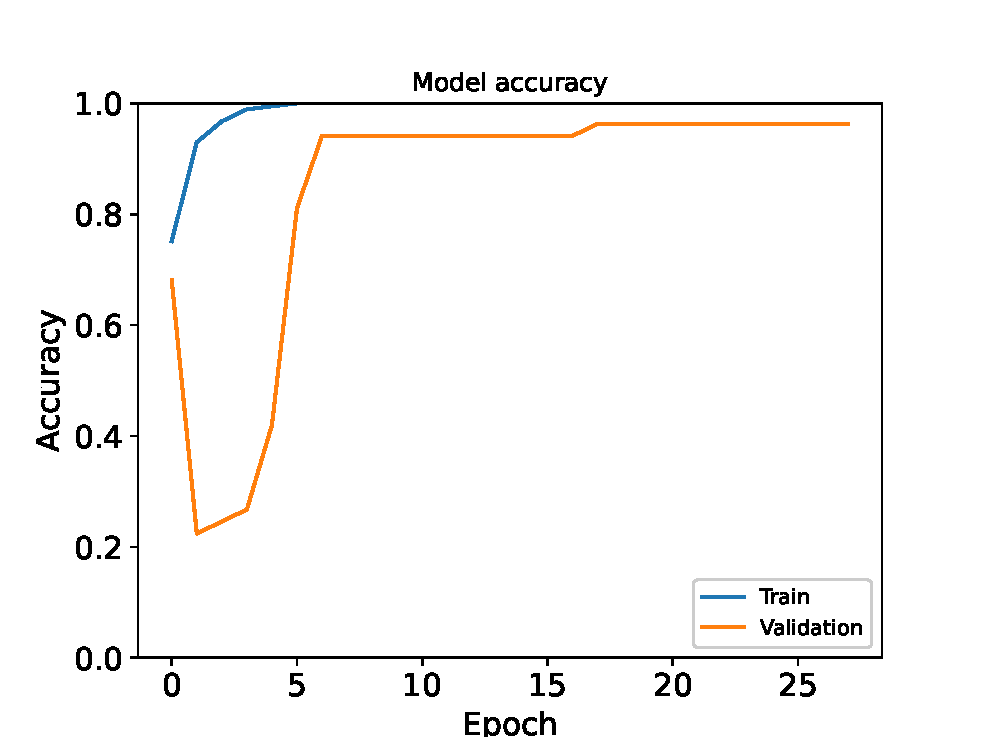
\includegraphics[width=\textwidth]{./fig/model4/accuracy4.eps}
        \caption{Accuracy of Model 4}
        \label{fig:model4_accuracy}
    \end{minipage}
    \begin{minipage}{0.45\textwidth}
        \centering
        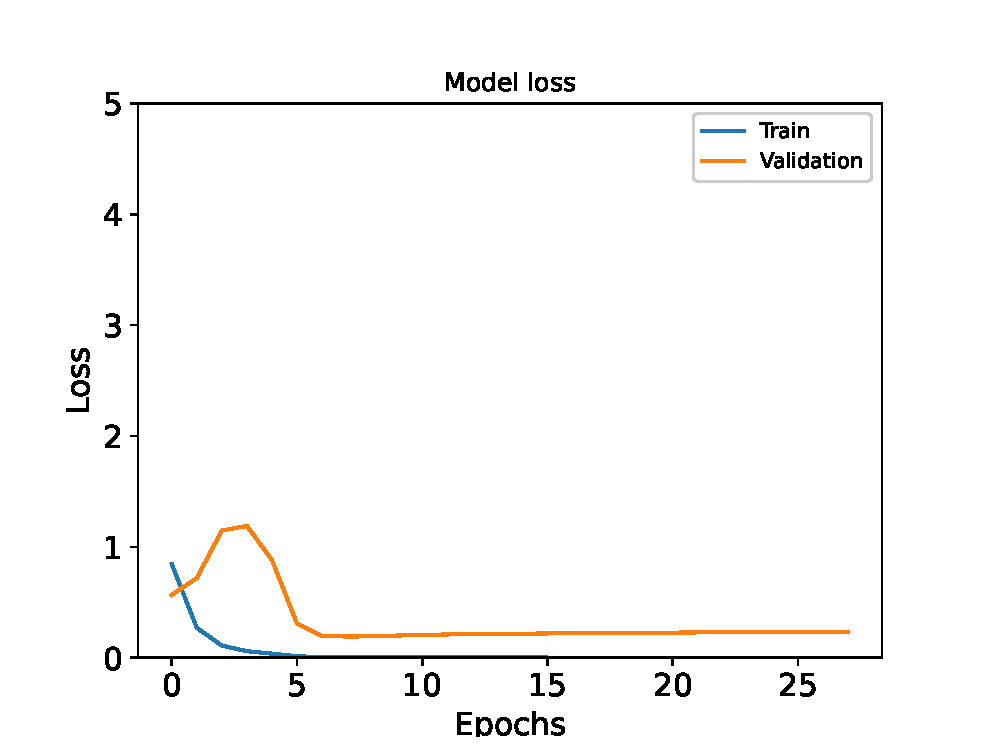
\includegraphics[width=\textwidth]{./fig/model4/loss4.eps}
        \caption{Loss of Model 4}
        \label{fig:model4_loss}
    \end{minipage}
\end{figure}

Observations of training accuracy and loss over time indicate a significant improvement in model performance. Both training and validation accuracies approach 1, with validation losses dropping to around 0.2, suggesting strong generalization capabilities. This indicates that the model not only excels on training data but can also generalize effectively to new, unseen data.

\textbf{Re-Evaluating Accuracy on the Test Set}

The updated model is then re-evaluated on the test set, with results as \autoref{tab:model_accuracy2}:

\begin{table}
    \centering
    \caption{Model 4 accuracy on the test set}
    \begin{tabular}{cccccc}
        \toprule
        & normal & horizental\_line & vertical\_line & slope & other \\
        \midrule
        accuracy(\%) & 98.4 & 96.7 & 85.6 & 96.5 & 96.5 \\
        \bottomrule
    \end{tabular}
    \label{tab:model_accuracy2}
    \end{table}

Comparing the accuracy before and after changing the resolution, there is a noticeable improvement, though it is not substantial. This modest increase could be attributed to the already high accuracies nearing 1, where further improvements have diminishing returns.

The results affirm the potential benefits of processing higher-resolution images, particularly in settings demanding high fidelity and detail, such as biological tissue analysis and research.

\subsection{Investigating the Optimal Cutting Angle for the Machine}

In order to determine the optimal cutting angle for the microtome, images of tissue sections cut at various angles ranging from 8 to 12 degrees, at 0.5-degree increments, were prepared. Each angle category consisted of 100 images, resulting in a total of 9 distinct groups of data. Model 4 was then utilized to assess the quality rate of each group, aiming to identify the angle at which the highest yield of quality sections was achieved.

The table and graph below present the accuracy, defined as the percentage of high-quality cuts, for each cutting angle:

\begin{figure}[htbp]
    \centering
    \begin{minipage}{0.4\textwidth}
        \centering
        \captionof{table}{Normal accuracy on different angles}
        \begin{tabular}{cc}
            \toprule
            Angle & Accuracy(\%) \\
            \midrule
            8 & 80 \\
            8.5 & 81.5 \\
            9 & 83.5 \\
            9.5 & 93.3 \\
            10 & 96.6 \\
            10.5 & 88.8 \\
            11 & 84.2 \\
            11.5 & 66.6 \\
            12 & 62.2 \\
            \bottomrule
        \end{tabular}
        \label{tab:model_accuracy_angle}
    \end{minipage}
    \begin{minipage}{0.55\textwidth}
        \centering
        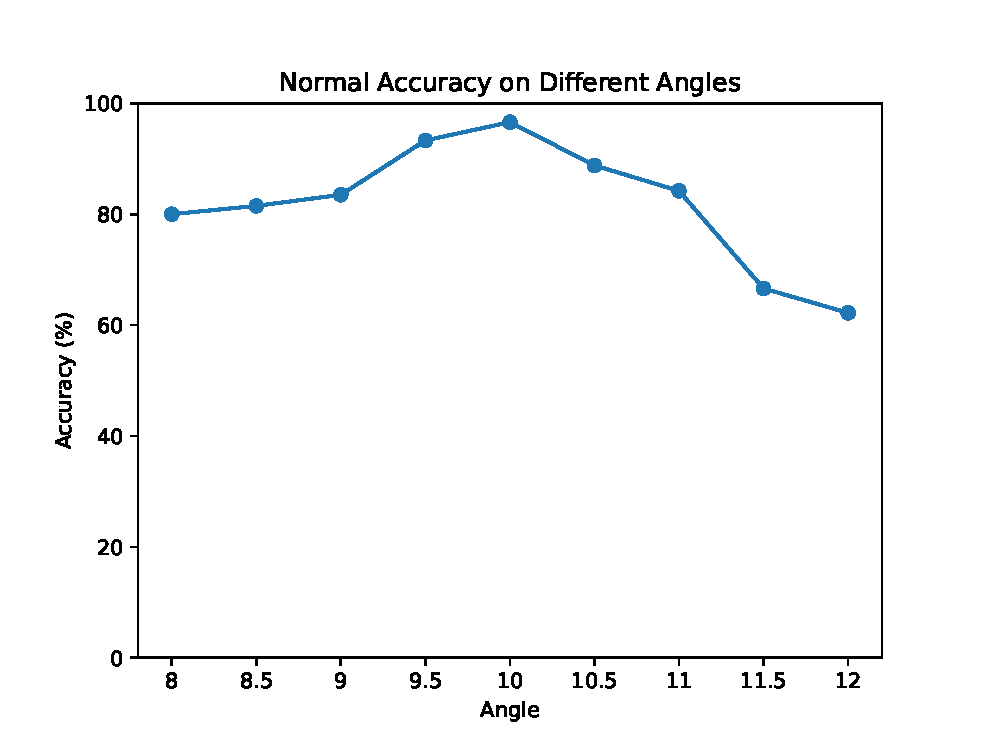
\includegraphics[width=\textwidth]{./fig/assistplot/angle_accuracy.eps}
        \captionof{figure}{Model Accuracy on Different Angle}
        \label{fig:angle_accuracy_histogram}
    \end{minipage}
\end{figure}

From the data presented in \autoref{tab:model_accuracy_angle}, it is evident that the optimal cutting angle for achieving the highest yield of quality tissue sections is 10 degrees, which demonstrates an impressive 96.6\% accuracy.

Additionally, as illustrated in \autoref{fig:angle_accuracy_histogram}, to maintain a section quality rate of at least 80\%, the cutting angle should be set between 9 and 10.5 degrees. This range not only ensures a high rate of quality cuts but also offers some flexibility in machine settings to accommodate possible variations in tissue type or condition.


\subsection{Model Generalizability}

The experiments thus far have utilized ovarian tissue sections from fish. In practical applications, we may encounter diverse tissue samples, including other organs or specimens from different animals. Therefore, it's crucial to assess the generalizability of our model across various tissue types.

A new dataset comprising fish lung tissue sections has been prepared, categorized into four classes: good, normal, bad, and other. These categories are demonstrated in the figures below:
(as shown in \autoref{fig:fish_lung})


\begin{figure}[H]
    \centering
    \begin{minipage}{0.24\textwidth}
        \centering
        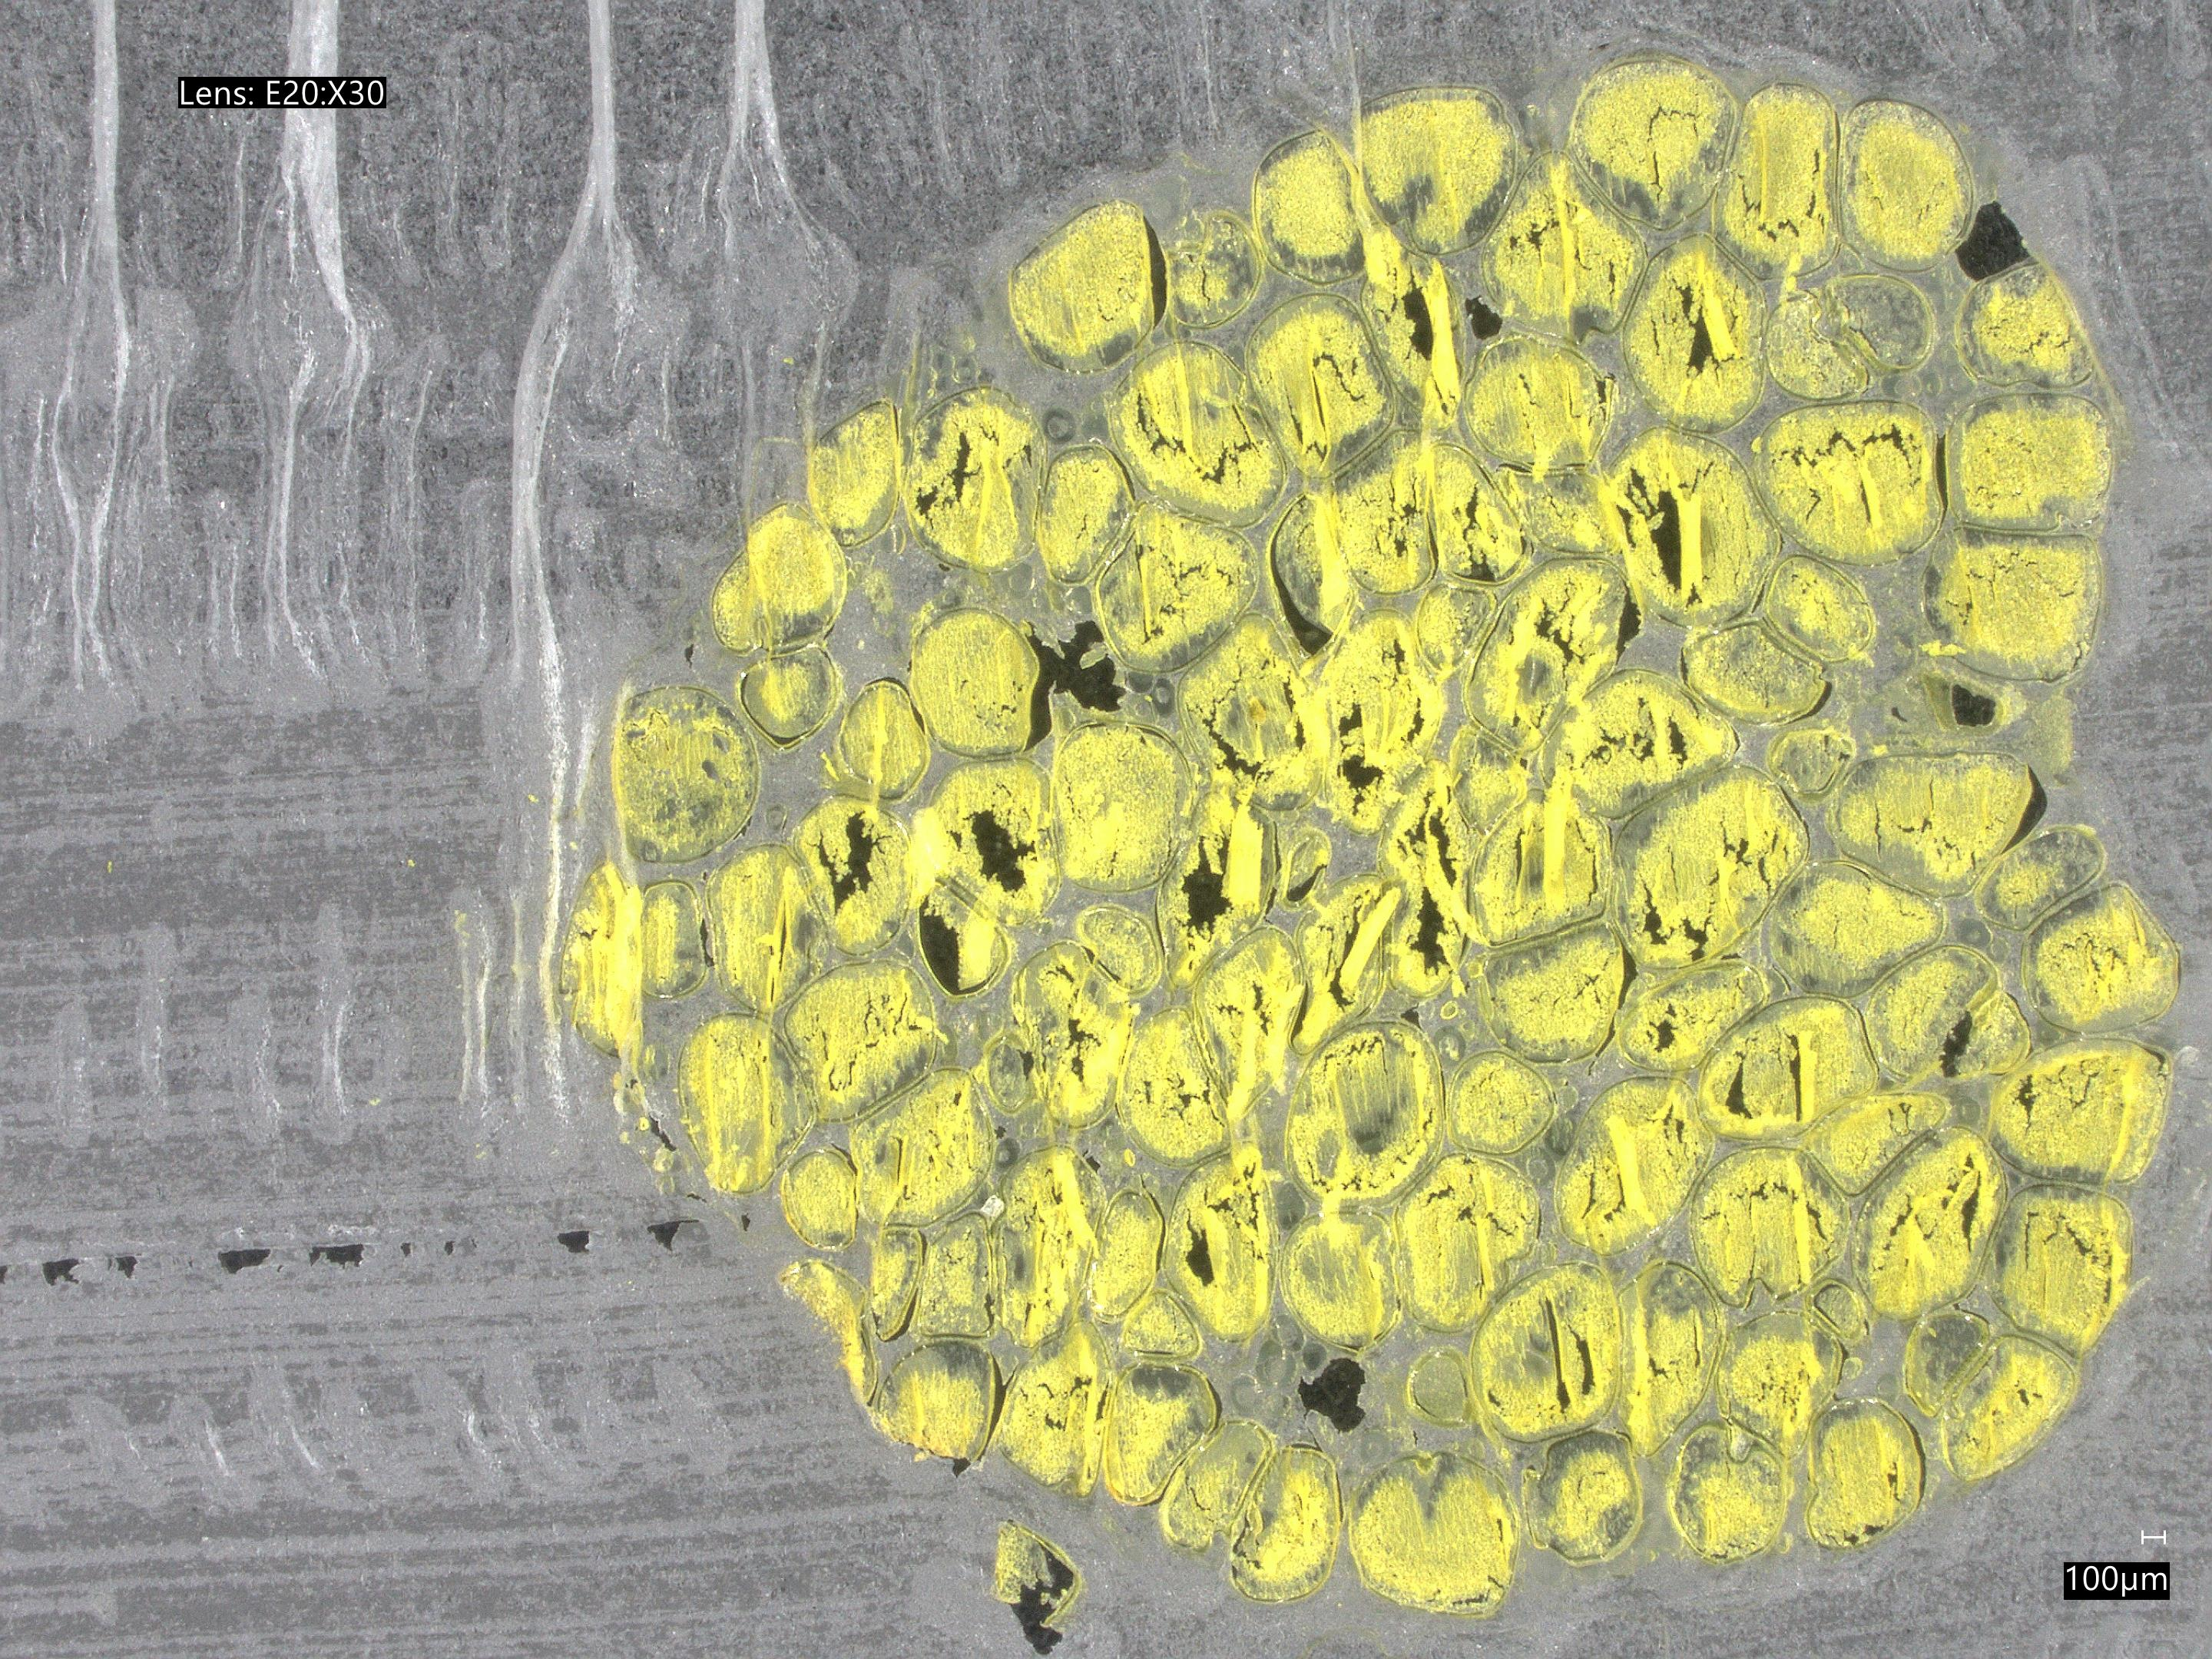
\includegraphics[width=\textwidth]{./fig/fish_lung/good20240313_144138.jpg}
        \caption*{Good}
        % \label{fig:good_fish_lung}
    \end{minipage}
    \begin{minipage}{0.24\textwidth}
        \centering
        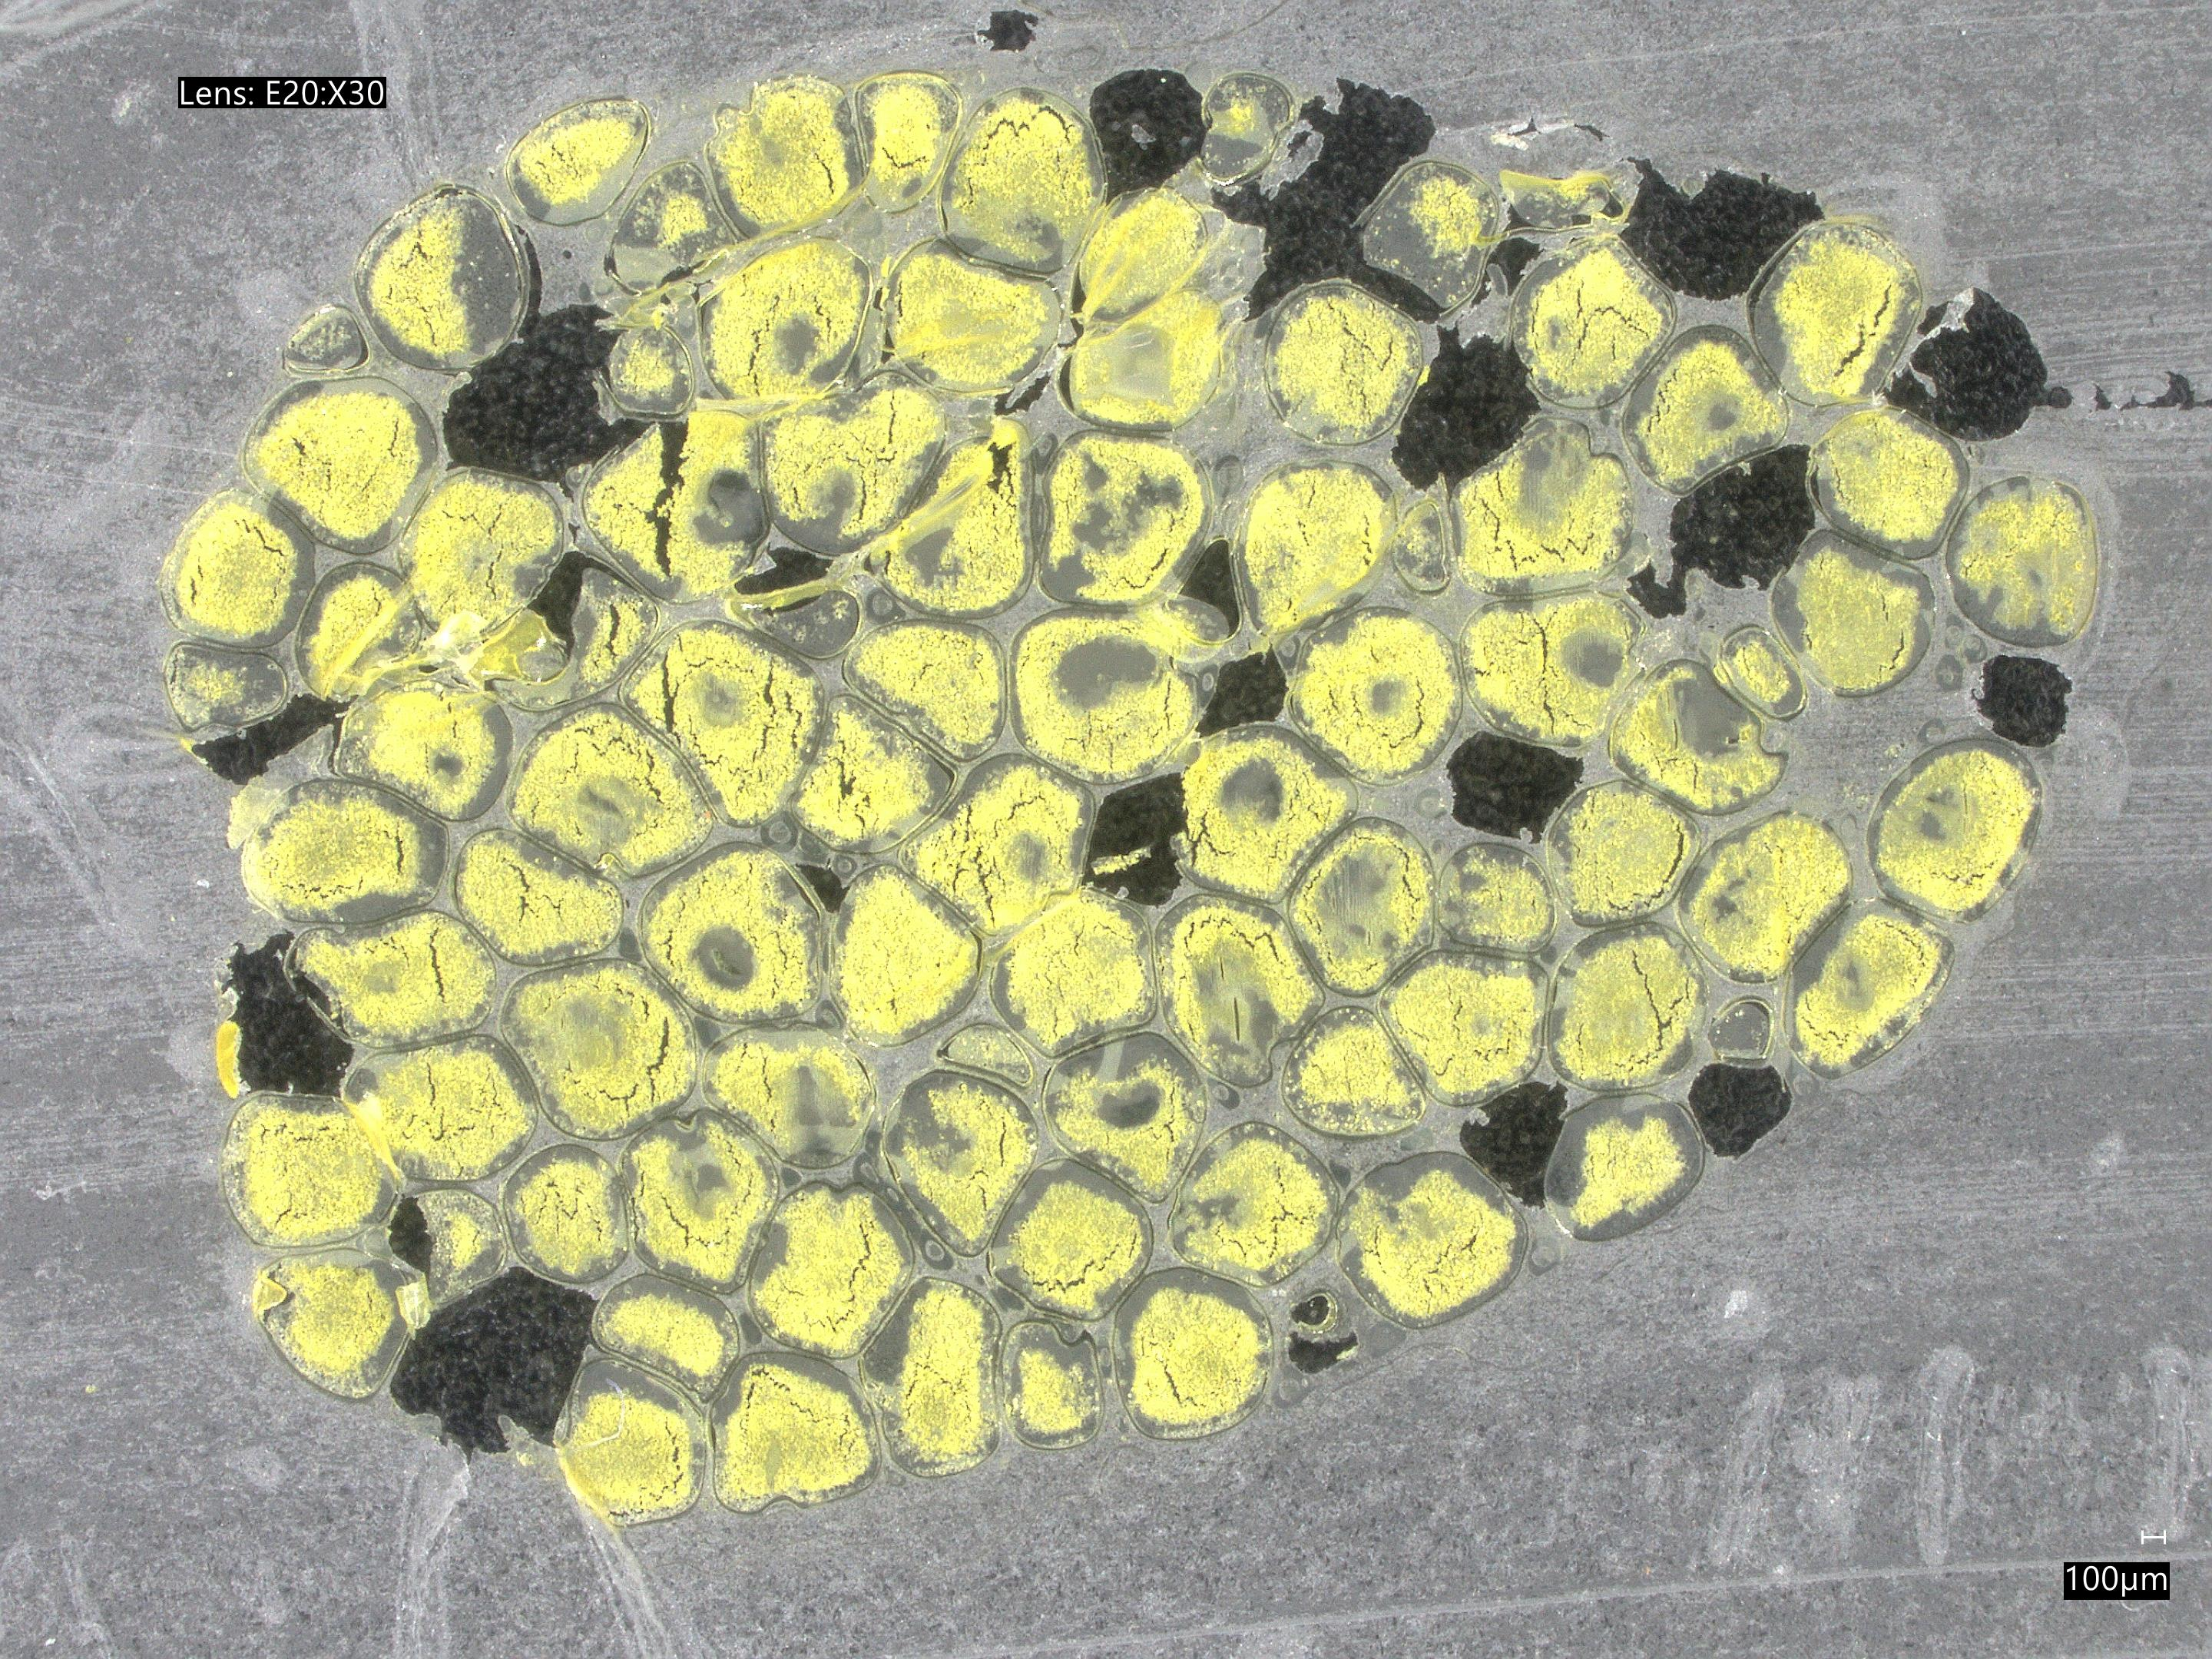
\includegraphics[width=\textwidth]{./fig/fish_lung/normal20240313_141726.jpg}
        \caption*{Normal}
        % \label{fig:noraml_fish_lung}
    \end{minipage}
    \begin{minipage}{0.24\textwidth}
        \centering
        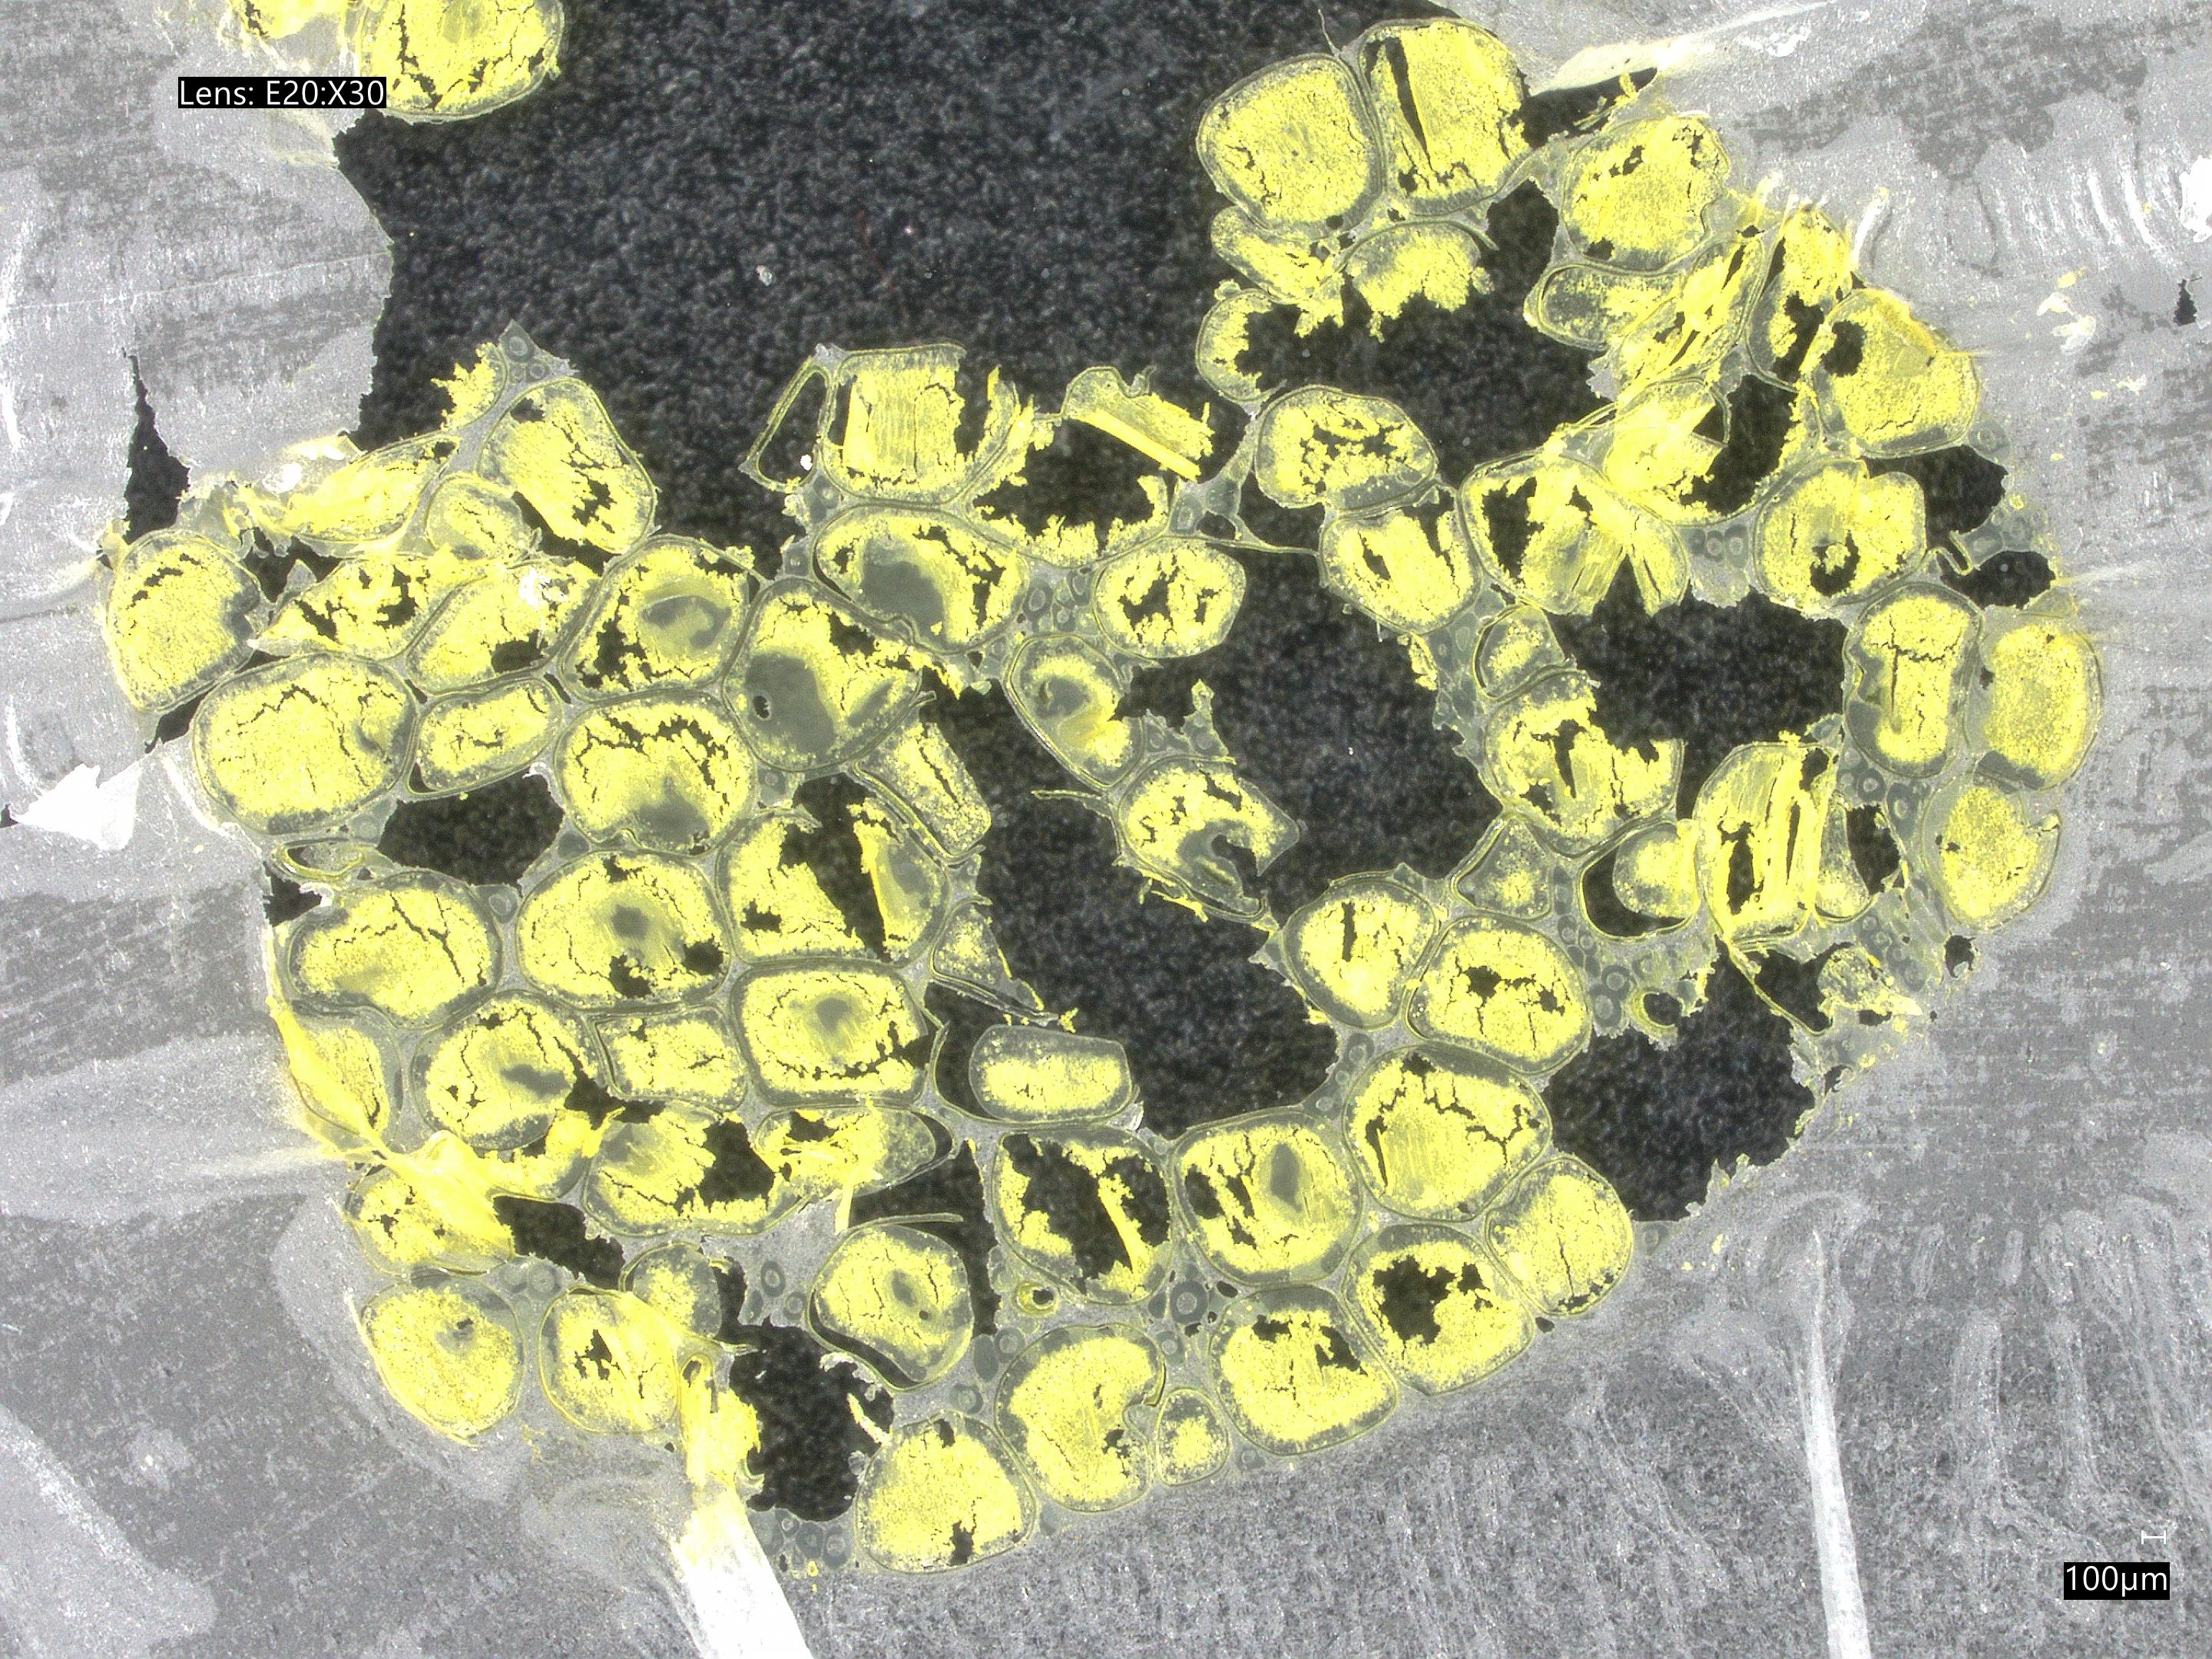
\includegraphics[width=\textwidth]{./fig/fish_lung/bad20240313_140952.jpg}
        \caption*{Bad}
        % \label{fig:bad_fish_lung}
    \end{minipage}
    \begin{minipage}{0.24\textwidth}
        \centering
        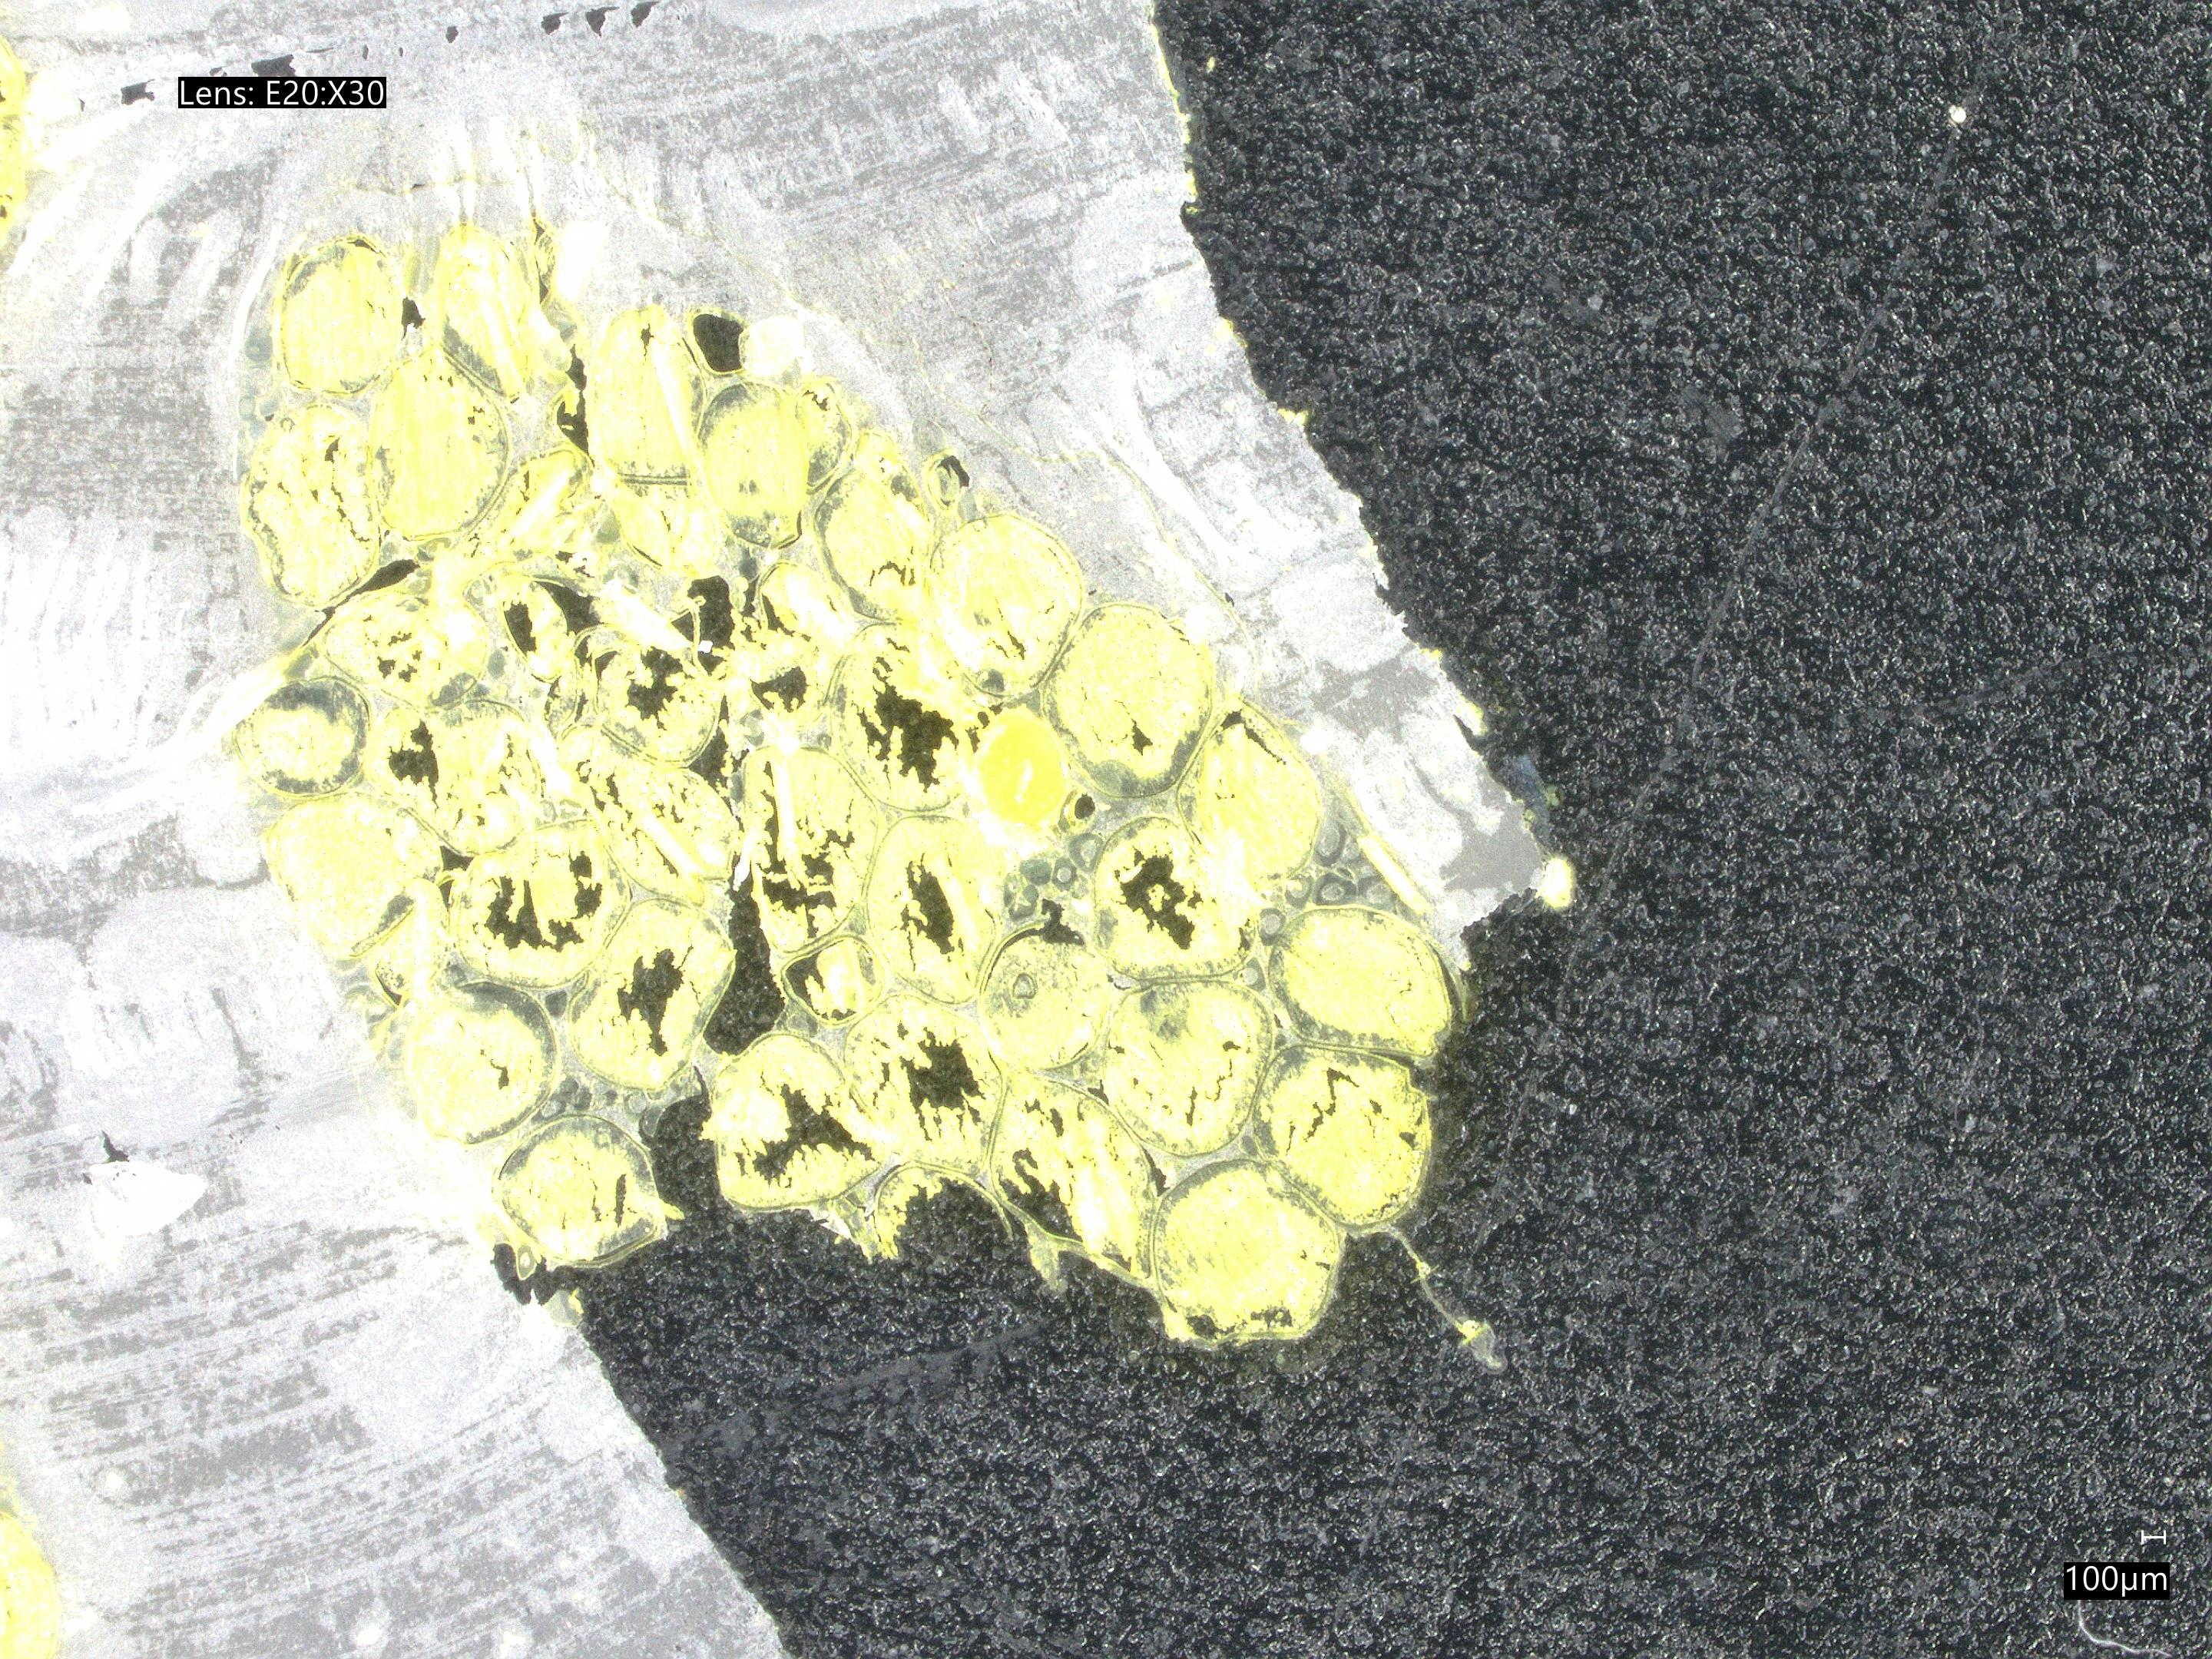
\includegraphics[width=\textwidth]{./fig/fish_lung/other20240313_141858.jpg}
        \caption*{Other}
        % \label{fig:other_fish_lung}
    \end{minipage}
    \caption{Four categories of fish lung tissue}
    \label{fig:fish_lung}
\end{figure}

The original model architecture (Model 4) is maintained but retrained with the fish lung images at a resolution of 1152x864. The training accuracy and loss are presented in the \autoref{fig:model5_acc} and \autoref{fig:model5_loss}.

\begin{figure}[H]
    \centering
    \begin{minipage}{0.45\textwidth}
        \centering
        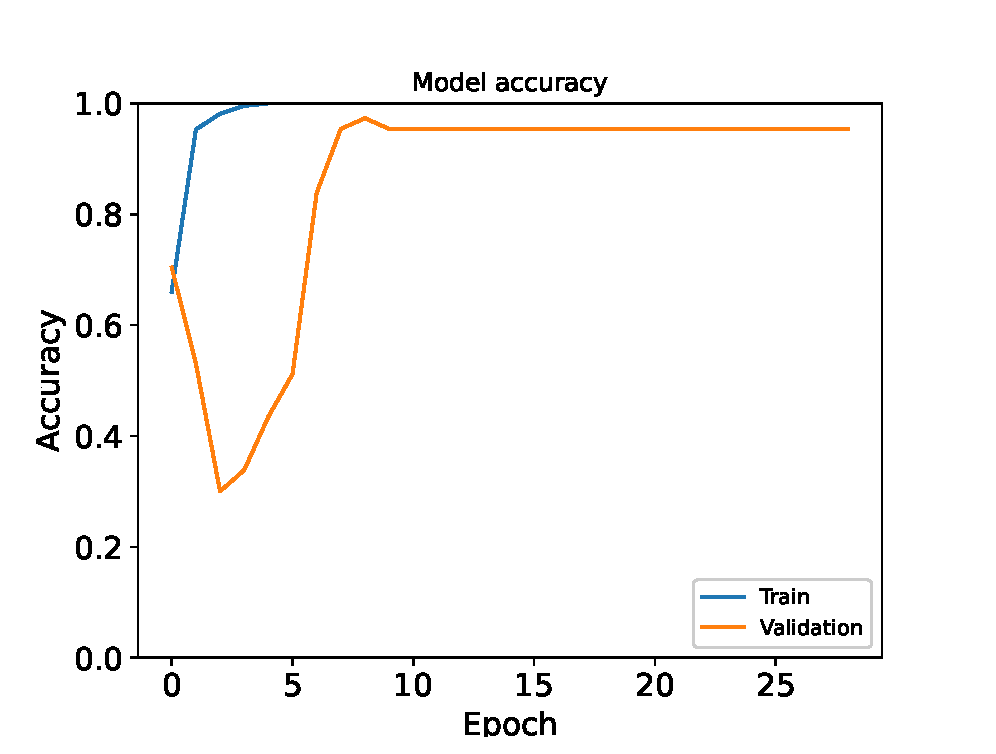
\includegraphics[width=\textwidth]{./fig/fish_lung/accuracy5.eps}
        \caption{Accuracy of Model 5}
        \label{fig:model5_acc}
    \end{minipage}
    \begin{minipage}{0.45\textwidth}
        \centering
        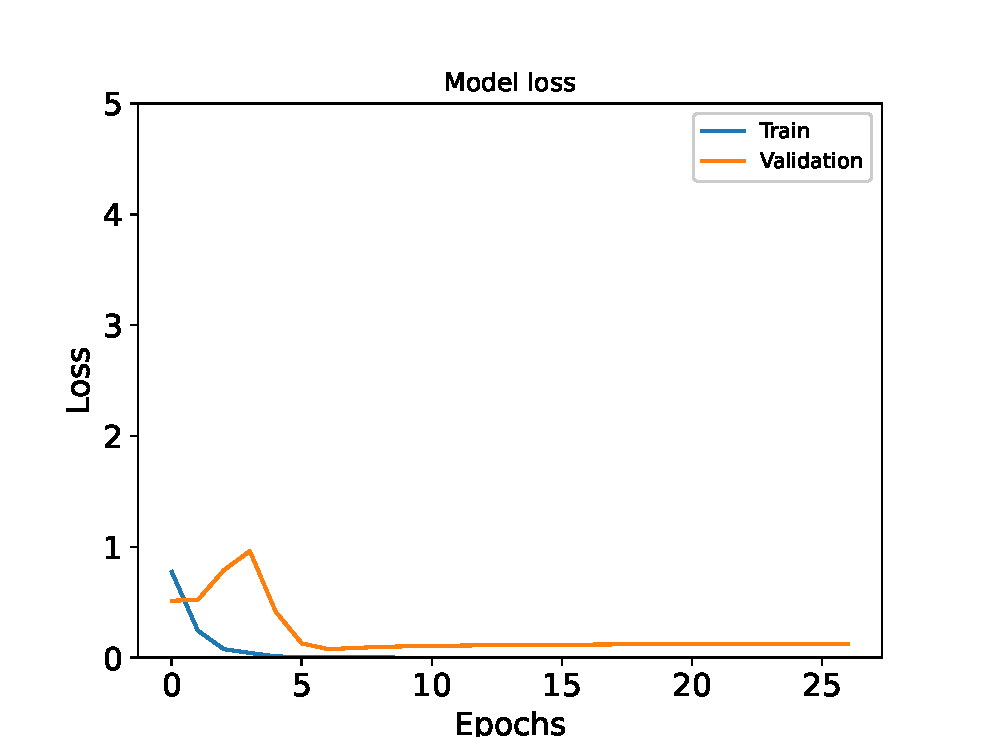
\includegraphics[width=\textwidth]{./fig/fish_lung/loss5.eps}
        \caption{Loss of Model 5}
        \label{fig:model5_loss}
    \end{minipage}
\end{figure}

The training and validation accuracy rapidly increase and maintain high levels, indicating robust model performance on both datasets. The loss plot shows a rapid decline in training loss towards zero, with validation loss stabilizing after an initial spike—suggesting good fit and generalization.

The model is further tested on a test set, and the results are shown in \autoref{fig:accuracy_histogram2}.

\begin{figure}[H]
    \begin{minipage}{0.45\textwidth}
        \centering
        \captionof{table}{Model accuracy on the test set}
        \begin{tabular}{ccccc}
            \toprule
            label & accuracy(\%) \\
            \midrule
            bad & 94.1 \\
            good & 98.2 \\
            normal & 94.7 \\
            other & 95.0 \\
            \bottomrule
        \end{tabular}
        \label{tab:model_accuracy3}
    \end{minipage}
    \begin{minipage}{0.45\textwidth}
        \centering
        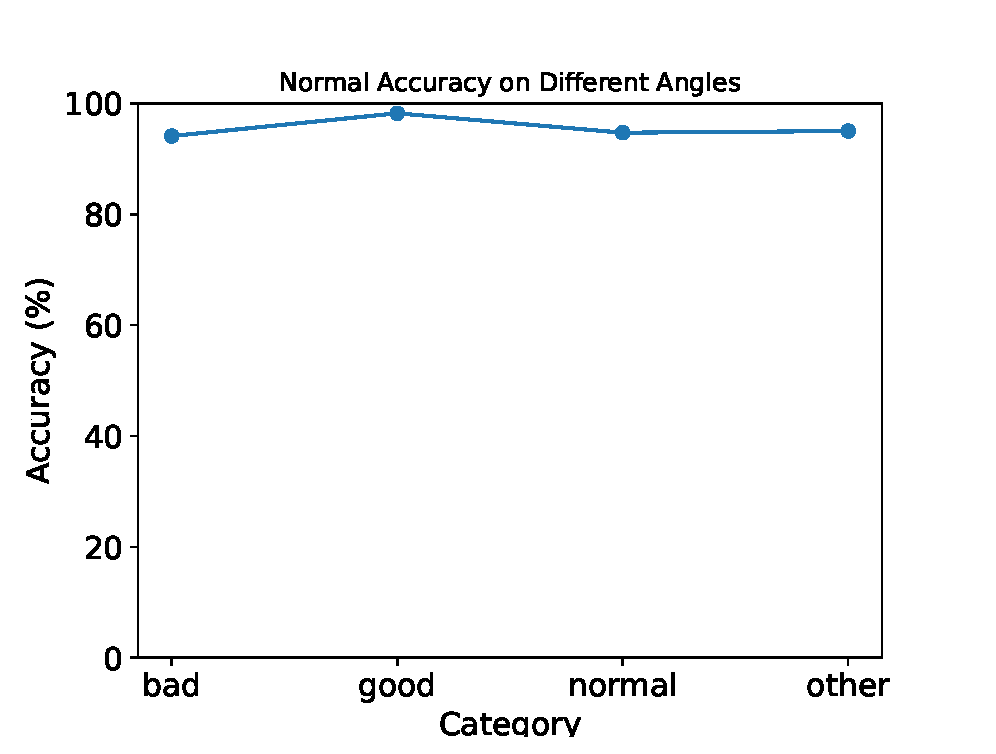
\includegraphics[width=\textwidth]{./fig/assistplot/angle_accuracy2.eps}
        \caption{Model Accuracy on Test Set}
        \label{fig:accuracy_histogram2}
    \end{minipage}
\end{figure}

The model demonstrates over 90\% accuracy across all labels, indicating its strong performance and substantial generalizability. This suggests that the model can effectively classify different types of tissue sections, potentially making it a versatile tool for various biomedical imaging applications.
The robustness of the model across different tissue types underscores its potential in tissue quality assessment and classification tasks.

